 % Copyright (c) 2016 Ongun Kanat <ongun.kanat@gmail.com>
% This document is a free software licensed under MIT license.
% For redistribution details look at COPYING file.

% 12pt and ISO A4 paper with title page add notitlepage for otherwise
\documentclass[a4paper, 12pt, titlepage]{article}

% 2cm margin from all sides
\usepackage[a4paper,margin=2cm]{geometry}
\usepackage{pythonhighlight}
% Use American English for dates etc.
\usepackage[american]{babel}
% If document is in Turkish then use
% \usepackage[turkish]{babel}
% or for both
% \usepackage[turkish,american]{babel}
\usepackage{movie15}
% in documenet

% Indent at section beginnings
% \usepackage{indentfirst} % look at below for reverse
% Paragraph spacings set parindent to 0
\setlength{\parindent}{0pt}
\setlength{\parskip}{12pt}

% utf-8 support
\usepackage[utf8]{inputenc}

% Graphics for PDFTeX
\usepackage[pdftex]{graphicx}

% Figure placement
\usepackage{float}

% An enumeration package for flexible enumeration
\usepackage{enumitem}

% Courier monospace font
\usepackage{courier}

% Links, both local and external
\usepackage{hyperref}
\hypersetup{
	unicode=true,
	colorlinks=true,
	urlcolor=blue,
	citecolor=black,
	menucolor=black,
	linkcolor=black
}

% Figure captions are bold
\usepackage[labelfont=bf]{caption}

% Pseudocode
\usepackage{algorithmicx}
\usepackage{algpseudocode}
\usepackage{algorithm}

% Syntax highlighting simple
\usepackage{listings}
\usepackage{amsmath}
\lstset{basicstyle=\ttfamily,frame=lines,tabsize=4}
\renewcommand{\lstlistingname}{Code}

% Syntax higlighting (advanced)
%\usepackage{minted}

% Title, author and date info
\title{My Glorious Report}
\author{Besim Ongun Kanat \\ 150120000}
\date{December 22, 2016}

\begin{document}
% Fix Turkish fix hypenation
%\shorthandoff{=}

% For a generic title page one can use standard \maketitle command
% It will use the title info above
% \maketitle

% The title page can be made by hand as below
\begin{titlepage}
	\begin{center}
		\large{Istanbul Technical University \\ Faculty of Computer and Informatics \\ Computer Engineering Department} \\
		\vspace{150pt}
		\Large{BLG 354E \\Signals \& Systems for Computer Engineering  \\Homework I}  \\
		\vspace{30pt}
		\large{Uğur Uysal - 150140012} \\
		\vspace{\fill} % Fill out until the page end
		\large{March 9\textsuperscript{th}, 2018}
	\end{center}
\end{titlepage}
\pagenumbering{roman}
\newpage
\tableofcontents
\newpage

% For the ones who doesn't know: 1,2,..9 called West Arabic numbers
\pagenumbering{arabic}
\section{Question I}
\begin{figure}[H]
	\centering
	\caption{Diagram of taking photo and projecting it. }
	\label{fig:Graphic}
	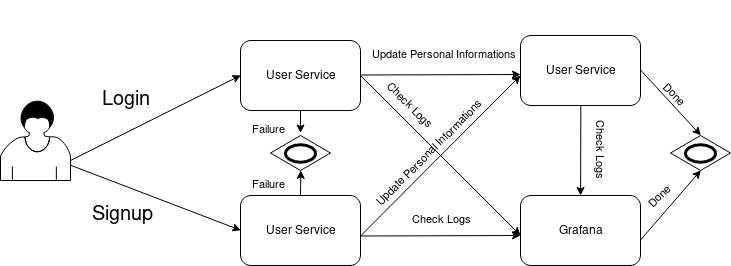
\includegraphics[scale=0.3]{Untitled Diagram.pdf} % scale 75%
\end{figure}

\section{Question II}
\paragraph{} The heartbeat records is a signal transformed from analog to digital in this example. Heart is periodically beating and it creates oscillation and it is a signal actually.
\paragraph{} Voice record is same like heart beat but it does not have to periodic. Sound is oscillation of particles in the environment. It is signal too.
\paragraph{} Images are kind of representation of light in the digital environment by help of some techniques. It is also signal.
\section{Question III}
\begin{center}
Roots are \\
$ z_1 = -\sqrt[8]{-1} $ \\
$ z_2 =  \sqrt[8]{-1} $\\
$ z_3 = -(-1)^{\cfrac{5}{8}} $\\
$ z_4 =  (-1)^{\cfrac{5}{8}} $
\end{center}

\section{Question IV}
\begin{center}
    Taylor Expansion of $ e^{x}$ \\
    $ e^{z} = \sum_{n=0}^{\infty }{\cfrac {z^{n}}{n!}} $ \\
$ e^{ix} = 1+ ix + \cfrac{(ix)^{2}}{2!} + \cfrac{(ix)^3}{3!} $ \space ...\\
$ = 1+ ix - \cfrac{x^2}{2!} - \cfrac{ix^3}{3!} $ \space ... \\
Group them.. \\
$= (1-\cfrac{x^2}{2!}+\cfrac{x^4}{4!}-) + i*(x- \cfrac{x^3}{3!}+\cfrac{x^5}{5!}- )$ \\
$= \cos {x} + i\sin{x}$
\end{center}

\section{Question V}
\subsection{Part A - Odd Function}
\paragraph{}
Let's $ f(x) = y $ \space a function with one parameter. If $ f(x) = -f(-x) $\space we call them odd functions. For example $ \sin$\space is a odd function. $ \sin \pi = -\sin -\pi $
\subsection{Part B - Even Function}
\paragraph{}Let's $ f(x) = y $ \space a function with one parameter. If $ f(x) = f(-x) $\space we call them odd functions. For example $ \cos$\space is a odd function. $ \cos \pi = \cos -\pi $
\subsection{Part C - Matches}
$\sin \theta = \cos(\theta - \pi/2)$,\space $\cos(\theta + 2\pi k) = \cos \theta$\space if k is integer, $ \cos -\theta = \cos \theta$,
\space $ \sin -\theta  = - \sin \theta $,\space $ \sin(\pi k) = 0$\space if k is integer $ \cos(2\pi k) = 1$\space if k is integer, $ \cos(2\pi(k+1/2)) = -1$\space if k is integer.
\subsection{Part D - Derivations}
\subsection{i}
\begin{center}

$ \cos \theta =\cfrac{e^{i\theta}+e^{-i\theta}}{2}\, \sin \theta =\cfrac{e^{i\theta} - e^{-i\theta}}{2i}$ \\
$\cos ^{2} \theta + \sin ^2 \theta = \cfrac{e^{2i\theta }+ 2 + e^{-2i\theta}}{4} - \cfrac{e^{2i\theta } - 2 + e^{-2i\theta}}{4} = \cfrac{2-(-2)}{4} = 1$
\end{center}
\subsection{ii}

\begin{center}
    $\cos ^{2} \theta - \sin ^2 \theta = \cfrac{e^{2i\theta }+ 2 + e^{-2i\theta}}{4} + \cfrac{e^{2i\theta } - 2 + e^{-2i\theta}}{4}$ \\
$ = \cfrac{2(e^{2i\theta} + e^{-2i\theta})}{4} =  \cos 2 \theta $
\end{center}
\subsection{iii}

\begin{center}
    $2 \sin \theta \cos \theta = 2* \cfrac{e^{i\theta}+e^{-i\theta}}{2} * \cfrac{e^{i\theta}-e^{-i\theta}}{2i} $ 
$ = \cfrac{2(e^{2i\theta} - e^{-2i\theta})}{4i} =  \sin 2 \theta $
\end{center}
\subsection{iv}
\begin{center}
From Euler expansion arithmetic operations.
\end{center}
\subsection{v}
\begin{center}
From Euler expansion arithmetic operations.
\end{center}
\section{Question VI}
\begin{center}
$ \sum_{k=1}^{N}{A_k\cos(\omega t +\theta)}  = \sum_{k=1}^{N}{ \operatorname {Re} \{ A_k e^{j\omega_0 t + \phi_k } } \} $ \\
$ = \operatorname {Re} \{ \sum_{k=1}^{N}{A_k e^{j\phi_k} e^{j\omega_0 t} } \} $ \\
$ = \operatorname {Re} \{ ( \sum_{k=1}^{N}{A_k e^{j\phi_k}  }) e^{j\omega_0 t} \} $ \\
$ = \operatorname {Re} \{ (A e^{j\phi})e^{j\omega_0 t} \} $ \\
$ = \operatorname {Re} \{ (A e^{j(\omega_0 t + \phi )} \} $ \\
$ A = cos(\omega_0 t + \phi)$
\end{center}
\section{Question VII}
\subsection{Part I}
\begin{center}
    $ z_1(t) = \cos(\omega t - \pi / 3), z_2(t) =3\sin(\omega t - \cfrac{5}{4}\pi) =
3\cos(\omega t - \cfrac{7}{4}\pi), z_3(t) = 2\cos(\omega t  4.7124)$
$x(t) = z_1(t) +z_2(t) + z_3(t) $ \\
$ e^{-\pi j/3} + e^{-7\pi j/4} +e^{-3\pi j/2j} $ then we can sum phasors like vector sum. \\ 
Result is $ r=1.47, \theta = 34.86 \text{\space} degree, 0.60 \text{\space} rad$, I used calculator for it.  \\
$ x(t) = 6\cos (\omega t - 0.19\pi)$
$ $
\end{center}
\subsection{Part II}
\begin{figure}[H]
	\centering
	\caption{Polar Coordinates of Phasors, created by wolframalpha }
	\label{fig:Graphic}
	\includegraphics[scale = 0.5]{Phasors.pdf} % scale 75%
\end{figure}

\subsection{Part III}
\begin{figure}[H]
	\centering
	\caption{500 hz frequency cosine signal with $0.19\pi$ phase (x axis time)}
	\label{fig:Graphic}
	\includegraphics[scale = 0.2]{sinosioid.pdf} % scale 75%
\end{figure}
\section{Question VIII}
    \subsection{Part I}
    \subsection{Part II}
The signal is periodic because we can find $ f_0 = gcd(f_k) $ \space and $f_0$\space is an integer. $ f_0 = 5 $ for this case and period is $ t_0 = \cfrac{1}{f_0} = 0.2 $

\subsection{Part III} 
The fundamental frequency $f_0 = 5 $ 
\section{Question IX}
    Multiplication of sinusoids..
    \subsection{Part I}
    \subsection{Part II}
    \subsection{Part III}
    $-7\cos(9990 \pi t + \pi/6) + -7\cos(10010 \pi t + \pi/6) $
\section{Question X}
We can take integral of products of functions.
If two functions satisfy this  $\int_{}{}{f(x)g(x)dx} = 0$  we called them as orthogonal functions. 
From Euler expansion arithmetic operations.
We can user Euler expansion for make the integral easy may be I am not even sure.
\section{Question XI}
It occurs when we are calculating sum of Fourier series. It makes jumps that can be seen at figure below.
 
Photo taken from Wikipedia article about  Gibbs phenomenon.\\
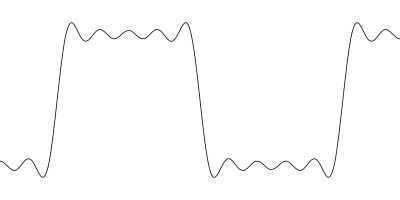
\includegraphics{gibs.png}



\end{document}
